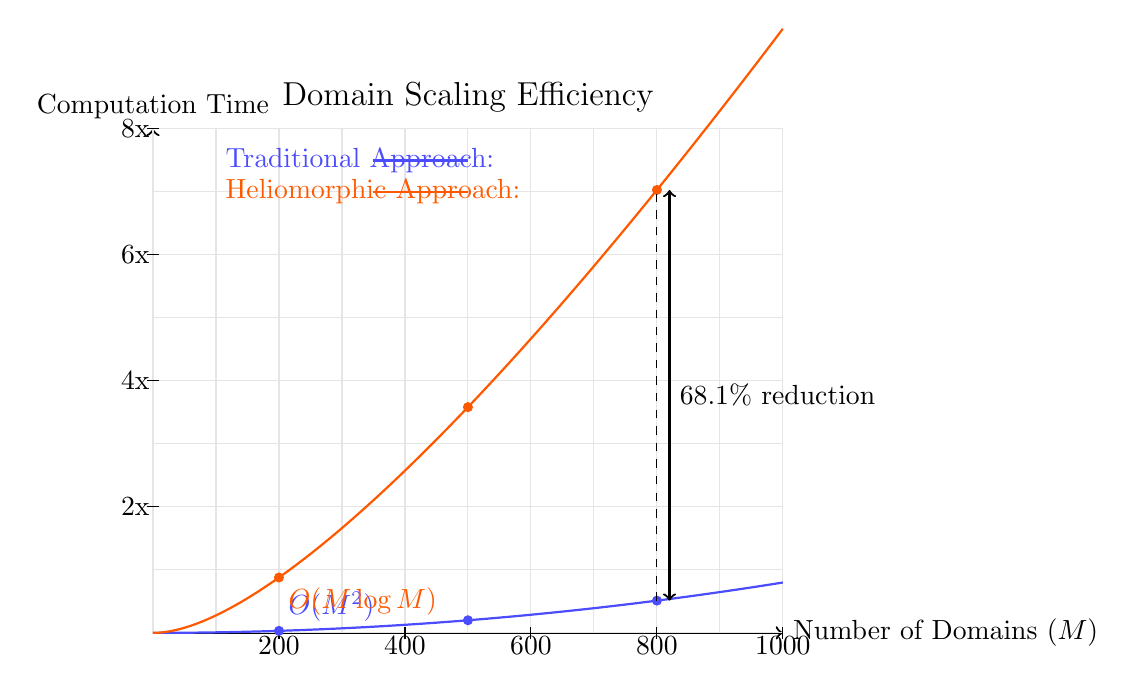
\begin{tikzpicture}[scale=0.8]
  % Define colors
  \colorlet{traditional}{blue!70}
  \colorlet{heliomorphic}{orange!70!red}
  
  % Set up axes
  \draw[thick, ->] (0,0) -- (10,0) node[right] {Number of Domains ($M$)};
  \draw[thick, ->] (0,0) -- (0,8) node[above] {Computation Time};
  
  % Grid
  \draw[gray!20] (0,0) grid (10,8);
  
  % X-axis labels
  \foreach \x in {2,4,...,10} {
    \draw (\x, -0.1) -- (\x, 0.1) node[below] {$\x$00};
  }
  
  % Y-axis labels
  \foreach \y in {2,4,6,8} {
    \draw (-0.1, \y) -- (0.1, \y) node[left] {$\y$x};
  }
  
  % Traditional approach curve (quadratic)
  \draw[traditional, thick] plot[smooth, domain=0:10, samples=100] (\x, {0.008*\x*\x});
  
  % Heliomorphic approach curve (log-linear)
  \draw[heliomorphic, thick] plot[smooth, domain=0:10, samples=100] (\x, {0.4*\x*ln(\x+1)});
  
  % Points marking specific values
  \filldraw[traditional] (2, {0.008*2*2}) circle (2pt) node[above right] {$O(M^2)$};
  \filldraw[heliomorphic] (2, {0.4*2*ln(2+1)}) circle (2pt) node[below right] {$O(M \log M)$};
  
  \filldraw[traditional] (5, {0.008*5*5}) circle (2pt) node[above right] {};
  \filldraw[heliomorphic] (5, {0.4*5*ln(5+1)}) circle (2pt) node[below right] {};
  
  \filldraw[traditional] (8, {0.008*8*8}) circle (2pt) node[above right] {};
  \filldraw[heliomorphic] (8, {0.4*8*ln(8+1)}) circle (2pt) node[below right] {};
  
  % Annotation of efficiency gap
  \draw[dashed] (8, {0.008*8*8}) -- (8, {0.4*8*ln(8+1)});
  \draw[<->, thick] (8.2, {0.008*8*8}) -- (8.2, {0.4*8*ln(8+1)}) 
    node[midway, right] {68.1\% reduction};
  
  % Legend
  \node[traditional, right] at (1, 7.5) {Traditional Approach:};
  \draw[traditional, thick] (3.5, 7.5) -- (5, 7.5);
  
  \node[heliomorphic, right] at (1, 7) {Heliomorphic Approach:};
  \draw[heliomorphic, thick] (3.5, 7) -- (5, 7);
  
  % Title
  \node[align=center, font=\large] at (5, 8.5) {Domain Scaling Efficiency};
\end{tikzpicture}